\chapter{INLOOM QT: A facility for quality testing INLOOM}

This chapter aims to present the design for a software, that allows for the validation
of the evaluations INLOOM \cite{1} produces. For this purpose, the requirements that are 
placed on the intended application are first compiled. The datasets that are available for 
the validation are analyzed and a data structure, to be employed by the application, is 
derived. Continuing to follow this data-driven approach, a possible design for the intended
application is presented.



\section{Software Requirements}

INLOOM is supposed to evaluate student submissions to modelling tasks. Since this evaluation
is to be done without further human supervision, the system must be tested thoroughly, to 
avoid grading students unfairly or in error. The maintainer of INLOOM must be enabled to get
an insight into the current quality of INLOOMs results and to quickly react to newly encountered
sources of error.

This leads directly to two leading requirements (RQ) for the software proposed here. 

\begin{itemize}
    \item[\textbf{RQ1}] The software must be able to automatically test the \textit{quality} 
    of the results INLOOM generates.
    \item[\textbf{RQ2}] It must be possible to present the results of the performed validation
    in an easily comprehensible way, to quickly gain insight about the current state of affairs.
\end{itemize}



\section{Available Data}

The biggest limitation for the test system is the availability of test data. Since the
complexity of solutions to modelling tasks cannot be predicted and there can be multiple 
correct solutions to the same task, the literature agrees, that the only feasible method 
of validating the evaluations, an automatic grading tool like INLOOM creates, is comparing
the automatic evaluation to a manual one, which was created for the same student solution.

The usefulness of faking student solutions for this purpose is limited. Any testing done,
using faked up data, would ultimately result in unit tests for the constraints. Thus, the 
only way to gain a reliable impression of the quality of INLOOMs results, is to use it
in a live scenario or to at least use real data for testing.

Since every other part of the design, depends on the underlying data structure, which in turn 
heavily depends on the data available, this leads to an obvious third requirement or rather an
important limitation for the software proposed here.

\begin{itemize}
    \item[\textbf{RQ3}] All tests must be performed using the data available.
\end{itemize}

As mentioned before, the data available consists of automatically generated evaluations
for already manually graded student solutions, as well as the respective manual evaluations,
in analog form. 

\begin{figure}[h]
    \caption{Abstracted workflow of the creation of manual and automatic evaluations. Rectangles
    mark data elements, while ellipses represent process steps. The rectangles marked in green, 
    represent the data available for testing purposes.}
    \centering
    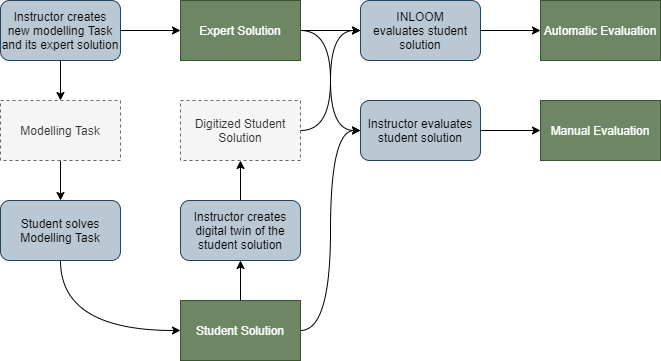
\includegraphics[scale=0.6]{graphics/AvailableData}
\end{figure}

\begin{itemize}
    \item[\textbf{RQ3.1}] The software must employ a data structure, that is able to hold
    information collected on automatic and manual evaluations and enables comparing the two.
\end{itemize}


\subsection{INLOOM Result Files}

The first part of the available data are the results produced by INLOOM. INLOOM persists its 
results in form of XML files. Each of the XML files, contains the results of the constraints 
applied to one student solution, as well as some meta data. The format used in these files,
has changed since the publication of \cite{1} and is now described by the following DTD:

\pagebreak
\lstset{language=XML}
\begin{lstlisting}[caption={
    XML format, currently used to persist the results the INLOOM software generates.
}, captionpos=b]
<!ELEMENT TestResult (TestData, Results, ResultPoints)>
<!ELEMENT TestData (ExpertModel, TestModel)>

<!ELEMENT ExpertModel EMPTY>
<!ATTLIST ExpertModel id CDATA #REQUIRED>

<!ELEMENT TestModel EMPTY>
<!ATTLIST TestModel id CDATA #REQUIRED>

<!ELEMENT MetaModel EMPTY>
<!ATTLIST MetaModel type CDATA #REQUIRED>

<!ELEMENT MCSIdentifier EMPTY>
<!ATTLIST MCSIdentifier id CDATA #REQUIRED>

<!ELEMENT MCSVersion EMPTY>
<!ATTLIST MCSVersion value CDATA #REQUIRED>

<!ELEMENT Results (CResult+)>

<!ELEMENT CResult (
    ExpertObject, ExpertType, TestObject, TestType
    Rule, Category, Points, Msg
)>
<!ELEMENT ExpertObject (#PCDATA)>
<!ELEMENT ExpertType (#PCDATA)> 
<!ELEMENT TestObject (#PCDATA)> 
<!ELEMENT TestType (#PCDATA)>  
<!ELEMENT Rule (#PCDATA)>  
<!ELEMENT Category (#PCDATA)>  
<!ELEMENT Points (#PCDATA)>  
<!ELEMENT Msg (#PCDATA)>  

<!ELEMENT ResultPoints (MaxPoints, TestPoints)>  
<!ELEMENT MaxPoints (#PCDATA)>  
<!ELEMENT TestPoints (#PCDATA)>  
\end{lstlisting}
\pagebreak

The root of the XML files is the "TestResult". All meta data is stored in "TestData", while
the individual constraint results are persisted as a list of "Result" under "Results".

Each such "Result" identifies the element, used during the constraint generation from the expert
solution, in "ExpertObject" and "ExpertType". The matching element of the student solution is
stored in "TestObject" and "TestType". The "Object" Part, holds the label or name of the used
element. The "Type" Part stores the type of the element in the diagram. What types INLOOM is able
to detect and grade, depends on the meta model used for the evaluation \cite{1}.

In the "TestData" branch, information about the evaluation is available. The "id" contained in 
"ExpertModel" references the expert solution the students work was compared to. "TestModel"
identifies the evaluated student solution. "MetaModel", "MCSIdentifier" and "MCSVersion"
contain versioning information about the created evaluation. These tags are interesting for 
making sure, that only evaluations, that were created under the same circumstances are compared.

The amount of test data sets will most probably not increase dramatically in the near future,
so there is no reason, to reduce the result data in any way before using it for testing. All
information required can automatically be extracted from the automatic evaluation result XML 
files.



\subsection{Manually Evaluated Student Solutions}

The second part of the test data are manual evaluations of student solutions. Thirty already
graded pen-and-paper student solutions to exam tasks were digitally reproduced by \cite{1}, to 
evaluate them using INLOOM. Of these thirty solutions, ten are solutions to exam tasks of the
summer term exams 2017, 2018 and 2019 respectively. Of the evaluations to this student solutions,
only an analog version exists. It should be noted that, that only the evaluations of the summer
term exam 2019 used the same uniform grading scheme for both the manual and automatic evaluation
by default \cite{1}. Every meaningful comparison of two evaluations requires the two to be 
based on the same grading scheme. This is the first formal limit (L) to the application.

\begin{itemize}
    \item[\textbf{L1}] The system requires manual and automatic evaluations as input, that were
    created, using the same grading scheme.
\end{itemize}

The literature agrees, that the manual evaluations of these digitized student solutions are 
the best evaluations known for the specific solution and therefore, are the only measure of 
quality one can apply to INLOOM. It can be assumed that the automatic evaluations quality is 
sufficient, if it reaches the same result as the manual evaluation. 

In order to compare these manual evaluations to the ones automatically generated by INLOOM 
however, they need to be digitized. Right now, the available manual evaluations consist of
a number of handwritten annotations in the student solutions. The annotations are mostly 
checkmarks and points awarded for elements of the model. What feature the annotation references
is indicated by its position in the student solution. Due to that format and the fact that the
student solutions were stored as black and white scans, it is unlikely that the evaluation data
can be automatically extracted. Therefor it is necessary to provide an evaluation digitization
facility.

\begin{itemize}
    \item[\textbf{RQ4}] The software must include a UI facility to digitize manually created 
    evaluations of student solutions. 
\end{itemize}



\subsection{Data Driven Data Structure}

There are some elements, automatic and manual evaluations obviously have in common. Others are
more oblique and some transformation is required, before they can be assumed present in both. 

Each of the evaluations, was made for exactly one \textit{student solution} to solve exactly one 
\textit{exercise}. Each evaluation can only ever be created by one \textit{evaluator} and 
using one \textit{expert solution} for reference. 

A comparison of an automatic and manual evaluation can thus be identified by a key, that consists
of the \textit{student id}, the \textit{exercise id} and the \textit{expert solution id}. There 
is no point in comparing an automatic evaluation to a manual one, if they differ in one of these
attributes. Such a comparison will later be called \textit{TestDataSet}. Both kinds of evaluation
need to contain these key attributes and rather obviously do.

For one student solution, there can exist multiple automatic and manual evaluations. Multiple
manual evaluators or different versions of the INLOOM software can create evaluations for 
the same student solution. The literature research showed, that it can be interesting to inspect
multiple manual evaluations of the same student solution, created by different evaluators. Each
evaluator has his/her own style and preferences, which will be reflected in the evaluation. 
Enabling the application to store multiple manual corrections of the same student solution 
allows for easy calculation of previously described \textit{clean scores} and any alike values. 

\begin{itemize}
    \item[\textbf{RQ3.2}] The software must be able to persist multiple evaluations for the 
    same student solution. 
\end{itemize}

Every expert solution is basically a collection of elements and features the student solution 
needs to contain, in order to be deemed correct. Both kinds of evaluation use an expert solution
for reference. For each expected feature the automatic evaluation adds a \textit{Result} to its
\textit{Results}-list. 

The equivalent in the manual evaluation are the point annotations. Each of those awards points
for a feature of the solution evaluated. A feature, that has to be part of an expert solution in
order for it to be correct. Each of the point annotations can thus be transformed into a "result"
of the manual evaluation. 

From the information collected about both the automatic and manual evaluations, using a data 
driven approach, a data structure can be inferred. Of the entities relevant to the system,
only two can exist without any dependencies. The \textit{Evaluator} and the \textit{Exercise}. 

For each exercise there can exist multiple \textit{ExpertSolutions}. As previously described, a
\textit{TestDataSet} must reference an \textit{Exercise}, an \textit{ExpertSolution} and a 
student, for it to be uniquely identifiable. 

For each \textit{TestDataSet}, or rather each combination of keys, that identify a 
\textit{TestDataSet}, there can exist multiple automatic and manual Evaluations: 
\textit{AutoEvals} and \textit{ManEvals}. Both of those are \textit{Evaluations} and generally
follow the format introduced by INLOOMs result XML files. The only difference between the two is,
that a manual evaluation must have been created by an \textit{Evaluator}, while for the creation
of an automatic evaluation the attributes \textit{MCSIdentifier} and \textit{MCSVersion} are 
required.

The following model results from combining all of these required features.

\begin{figure}
    \caption{Data model, that results from the structural analysis of the available data.}
    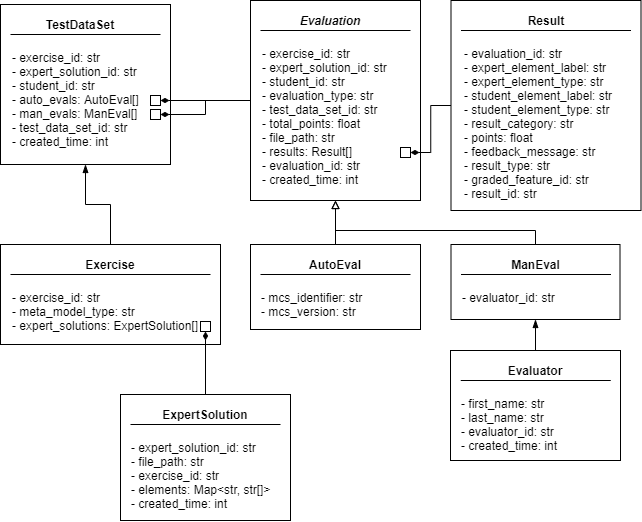
\includegraphics[scale=0.625]{graphics/Entities}
\end{figure}
\pagebreak



\subsection{Digitizing Manual Evaluations}

The need to digitize the manual evaluations before being able to compare them automatically
to the evaluations INLOOM produces, means a huge overhead for the testing process. 
Digitizing the manual evaluations is inevitable however. This is reflected by RQ4.
The effort required for digitizing manual evaluations must be reduced as much as possible.

The process of extracting the data from the manual evaluations into a data structure like the 
one presented above, can roughly be separated into three steps and is the same for each manual
evaluation.

\begin{enumerate}
    \item Supplying identifying attributes (exercise, student, expert solution).
    \item Supplying metadata (total points, evaluator).
    \item Transforming point annotations into results and adding those results to the evaluation
    until the point total is accounted for.
\end{enumerate}

Since many of the attributes, one needs to enter are repetitive and limited to a number of options,
the UI facility must aim to provide selections rather than inputs for as many of them as
possible. This can obviously be done for both the exercise and expert solution, since only a 
limited number of those are known to the application. The same holds true for the evaluator.

More interesting however, is easing the inputs required in the third step of the digitization, 
since it is the only one, that will have to be repeated multiple times. In each repetition of 
step three, six attributes need to be entered, in order to register a new \textit{Result} of 
the manual evaluation one is digitizing.  

\begin{enumerate}
    \item Expert Element Label
    \item Expert Element Type
    \item Student Element Label
    \item Student Element Type
    \item Result Category
    \item Points
\end{enumerate}

Of these only the student element label, student element type and points are not generic. The
rest of the attributes is limited to a number of options. The options, except the the ones 
for the result category, are defined by the employed expert solution. The options valid for 
use as a result category are defined by INLOOM and are immutable. Adding a new \textit{Result}
can thus be reduced to entering three values and selecting the rest from predefined options.



\section{KPI for Testing}

The literature research showed quite clearly, that a \textit{Grade Quotient Strategy} is 
the only real contender for any kind of statistic about the alikeness of two evaluations.
Since INLOOM is a constraint based system and its results need not be compared on a nominal
scale, it is not deemed necessary, to calculate any of the Inter-Rater-Reliability (IRR) 
statistics encountered in the literature. Assuming a nominal categorization, would disregard 
a big amount of the data available. 

Even when using a percentage difference for categories, artificially creating a nominal 
categorization, as was done in \cite{28} and thus enabling their employment, these statistics
do not add any significant new information. Also, their results are often less unintuitive 
than a simple quotient and are not deemed adequate, to provide a first glance impression of 
the current state of affairs. 

IRR are designed to mitigate, the effects of habitual and random decision making, when 
validating evaluations, that employ categories with ill defined options. A big part of the 
randomness, in the typical use cases of IRR, results from these ill defined options. 
Since the evaluator is required to make a judgement call, it is possible, that not even the
same evaluator will be able to repeat this decision, should (.*|they) be confronted with 
an alike case. This makes for grade equivalents in these evaluation, that can, by nature, not
be vindicated after the fact, since they are made up of partial decision, that can not be 
repeated with any amount of certainty.

The use case of INLOOM is quite different. As previously described the XML results of the 
system, list all the constraint results, the final grade is made up of. Thus, each step that
led to the final grade can be examined and it is most definitely possible to justify the final
grade and to repeat the evaluation.
For INLOOM one can conclude from its results, that the tool made an objectively wrong decision
during its evaluation. This is not the case in IRRs typical use cases and in those, one would
usually not be able to define \textit{objectively wrong}. 

Calculating IRR might still be interesting at a later point, since these statistics are 
employed in the literature and it might prove informative to be able to compare INLOOMs 
quality to the quality of other systems. 

IRR might also become interesting for INLOOMs use case, when more than one manual evaluation 
should be the norm rather than the exception, at some point in time. Under that circumstances 
IRR will become useful to compare multiple manual evaluations to one another and create 
something alike a clean score automatically.  

Since the software proposed here is required by RQ3.2, to be able to store multiple evaluations
of the same student solution, it is opportune to add another requirement, that ensures the 
possibility to calculate additional KPI later on.

\begin{itemize}
    \item[\textbf{RQ3.3}] The data collected by the proposed application must be easily 
    accessible to programmatic analysis, one might wish to perform on it in the future. 
\end{itemize}

Since this work aims to validate the quality of a constraint based system, with a uniform
output format, no meta analysis of the quality validation is required, to extract additional
information from a single value available. Instead of using meta statistics to extract more
information from the \textit{Grade Quotient}, due to the uniform output format of INLOOMs
result XML files, a more detailed analysis can be performed. As described earlier, data about
each constraints result is available. These results can be numerically analyzed in a number
of ways and on different levels of detail. A grade quotient equivalent can be calculated
and compared in each category and for each level of detail. Such an examination will enable 
the user of the proposed application not only to gain a quick overview over INLOOMs current
performance, but also enable (.*|them) to quickly identify likely sources of error. 



\subsection{Comparison Detail Levels}

A comparison of a manual and an automatic evaluation, collected and persisted as described, 
can happen on a number of different levels of detail, or rather with a number of different 
scopes. On each of these detail levels a number of categories has to be considered for 
comparison.

The final grade or exam score is the first and broadest category, two evaluations
can be compared in. The final grade is a rating, made up from a number of more detailed ratings
and does by itself not allow for an inspection of its composition. 
Each of the more detailed ratings is performed on, what in the literature is described as a 
\textit{MMU}, a \textit{minimal meaningful unit} \cite{28}. In INLOOMs case, these MMU are 
identified by the \textit{label} and \textit{type} keys of the result. INLOOM matches an MMU 
in the expert solution to one, identified in the student solution and, using constraints to 
compare their features, grades their alikeness. Each \textit{result} listed in INLOOMs result 
XML files, represents the result of one such rating. 

To evaluate the composition of the final grade, in a secondary analysis the results can be 
grouped by one of the available keys. By summing up the points of a group or evaluating the 
frequency of a certain result category within that group, one can calculate sub quotients of 
the grade quotient. These values specify the extent of agreement of two evaluations within a 
certain limit and are the most fine grained category for comparing two evaluations. 

Since both the automatic and the manual evaluation use the same expert solution to compare
the student solution to, the expert elements expected from the student solution are the 
same for both. Thus, it makes sense to use the expert elements as a key, for collecting data
on, since they are common to both the manual and automatic evaluations. 

Values collected for each evaluation, can be averaged over a group of evaluations. 
Such is interesting for both, combining multiple manual evaluations in a moderated evaluation
and for inspecting a group of related evaluations. Collections of evaluations for which an
average KPI can be evaluated, represent the third level of detail one can inspect INLOOMs 
results on.



\subsection{Categories of Comparison}

The main category of comparison, of the two evaluations will, as previously stated, be a regular
grade quotient. For each student solution, by the application identified using a key that 
consists of the student id, the exercise id and the expert solution id, such a quotient 
will be calculated as a result of the meta evaluation. Obviously such a grade quotient can 
be averaged over an arbitrary collection of evaluations later on.

Although more elaborate evaluations might prove interesting in the future, the application 
proposed here will only perform the most basic evaluation on the result level. In compliance
with RQ3.3 it will later easily be possible to extend the application by any evaluations 
that are feasible on the available datasets. 

In order to enable the user, to quickly identify sources of error, the application will group
found results by element type and sum up the points awarded to each group 
(\textit{points-per-element-type}). This way the user gets an easy grasp of where discrepancies
in the grade quotient originate. The comparison of the points-per-element-type rating can, just 
as the grade quotient, be expressed by a quotient per element type.

Evaluations will be grouped by evaluator and expert solution id. The grade quotient and 
points-per-element-type rating will be average over all evaluations within a group. 
The evaluator and expert solution id are obvious candidates for a comparison on this level 
of detail. 

As is expressed by the perceived need to employ IRR, evaluations by different reviewers can 
differ significantly. The application must take this into consideration and give the user the 
means to check for any negative effects using manual evaluations by multiple evaluators might 
have on the quality of the systems results. This is remedied by calculating an per evaluator
average of the alikeness ratings awarded to pairs of manual and automatic evaluations.

By calculating an average value for the evaluations of a specific expert solution, the user 
can examine INLOOMs results for error trends, that arise from the structure of a specific 
expert solution. 